\chapter{Introduction}

With new companies jumping into the Internet of Things (IoT),
major IT actors investing in the development of new
products~\cite{fortuneiot2019}, and telecoms operator building infrastructure
for the growing
demand\footnote{\url{https://www.proximus.be/en/id_cl_iot/companies-and-public-sector/it-services/iot/internet-of-things.html}},
it is fair to say that IoT caught the attention of many people and researchers
in the last years.
IoT technology allows the gathering of data and the control of actuators via
the Internet without any human interaction.
The field has been developed during the last decade and has maintained a
consistent growth since.
Business analysts agree that we can expect to reach at least 40 billion
installed IoT devices by 2027~\cite{businessinsider2020}.
We are already familiar with the traditional IoT products
we use in our households. Those products allow us to connect our light bulbs,
fridge, and washing machine to the Internet.
Meanwhile, the industrial usage of IoT, also known as industrial IoT (IIoT) is
one of the fastest-growing segments of the market.
More and more industries are adopting IIoT to consolidate their productions
with real-time monitoring, to organize predictive maintenance on their
assets and products to connect their supply chains, etc.
All of this is enabled with the help of sensor networks, and actuators, in a
wide variety of sectors like smart farming, smart cars,
smart cities, and energy management.

\paragraph{}

All these applications have in common that they rely on devices that
communicate wirelessly.
To suit this new demand, new communication protocols were created.
They can be classified by three different characteristics

\begin{itemize}
    \item Long or Short \emph{communication range}
    \item High or low \emph{data-rate}
    \item Low or high \emph{power usage}
\end{itemize}

Figure~\ref{fig:commrangegraph} shows the classification
of the existing wireless communication protocol used for the \emph{IoT} and
presents it in three main categories.

\begin{description}
    \item[Short-Range wireless communication] Short-range, high
        data-rate, low power
    \item[WiFi] relatively Short-range, high
        data-rate, high power consumption
    \item[Cellular communication] Long-range, high data-rate, high power
        consumption
    \item[Low-power wide-area network (LPWAN)] communication Long range,
        low power, and low data-rate
\end{description}

\begin{figure}[H] % TODO More info on axis
\centering
\begin{tikzpicture}
    \draw[->,thick] (-0.1,0)--(12,0) node[right]{Range};
    \draw[->,thick] (0,-0.1)--(0,8) node[above]{Data Rate};
    
    \node[draw] at (8,1.5) (lora) {LoRa};
    \node[draw] at (9.3,0.9) (sigfox) {SigFox};
    \node[draw] at (10,2) (nb) {NB-IOT};
    \node[draw,dotted,fit=(lora) (sigfox) (nb), label=above:{LPWAN}] {};

    
    \node[draw] at (2.2,3.5) (bluetooth) {Bluetooth};
    \node[draw] at (2.7,2.5) (zigbee) {ZigBee};
    \node[draw] at (2.0,1.8) (ble) {BLE};
    \node[draw] at (3,5) (wifi) {WiFi};
    \node[draw,dotted,fit=(bluetooth) (zigbee) (ble) (wifi), label=above:{Short-range}] {};

    \node[draw] at (7,5) (lte) {LTE};
    \node[draw] at (5.8,6) (5g) {5G};
    \node[draw,dotted,fit=(lte) (5g), label=above:{Cellular}] {};
\end{tikzpicture}
\caption{Comparison of the existing IoT wireless technologies by range and datarate}
\label{fig:commrangegraph}
\end{figure}


This work focuses only on \emph{LoRa}, a proprietary \emph{chirp spread spectrum}
modulation technique owned by \emph{Semtech}, operating in the sub-GHz
unlicensed Industrial, Scientific, and Medical (ISM) band\footnote{It is worth noting that Semtech also developed a version of LoRa that
operates in the 2.4GHz band but will not be covered in this text. When I will talk
about LoRa I will only talk about the version that operates on the sub-GHz ISM band.}.
I will cover LoRa in more detail in Section~\ref{section:lora}.
The main characteristics of \emph{LoRa} are its low power transmission and the
fact that it can trade data rate for range by fine-tuning the physical layer
(PHY) settings.
The long-range capabilities of the protocol caught the attention of
many people.
Hobbyists have succeeded in obtaining a record transmission distance of over 700 km with
a direct line of sight between the receiver and the
transmitter~\cite{network_2017}.
However, this case is not a real-world example. The range in urban areas is
around \emph{2 to 5 km} and around \emph{15 km} in suburban
areas~\cite{8030482}.

% \emph{LoRa} is often used in conjunction with an ALOHA based~\cite{loraalliance:lorawanspecification} MAC protocol deployed in a star-of-stars topology.
LoRa Wide Area Networks (LoRaWANs),
is composed of wireless \emph{motes} sending messages directly to \emph{gateways} (GWs).
Those GWs are connected to the internet and will relay messages to central servers
as we can see in Figure~\ref{fig:startopology}.
LoRa motes in a LoRaWAN use LoRA physical (Phy) layer in combination with a
random access Medium Access Control Protocol (MAC) called LoRaWAN as well.
This protocol is greatly inspired by ALOHA~\cite{loraalliance:lorawanspecification}.
Each mote can access the medium when a packet needs to be sent (random access)
and collision or packet damage is detected because the Ack will not arrive.
In that case, the mote backs off using a random wait time and retransmits.
Nodes only wake up their radio to send a packet and receive the Ack and can
sleep the rest of the time which realizes the low energy consumption.

This single-hop LoRaWAN topology has been successful because private (as well as public paid
services) LoRaWAN networks to connect to already exists
\footnote{\url{https://www.thethingsnetwork.org/map}}.
Private networks are deployable in contrast to other LPWAN like \emph{Sigfox} or \emph{NB-IoT}.

\begin{figure}[H]
\begin{subfigure}[b]{.5\textwidth}
    \centering
    \begin{tikzpicture}[auto, thick]
      % Place super peers and connect them
      \foreach \place/\name in {{(0,-1)/a}, {(2,0)/b}, {(2.5, -3)/c}}
        \node[gateways] (\name) at \place {};
      \node[server] (d) at (1.5,-1.5) {};
      %
      \foreach \source/\dest in {a/d, b/d}
        \path[dotted] (\source) edge (\dest);
      \path (c) edge (d); % Non dotted
      %
      % Place normal peers
      \foreach \pos/\i in {above right of/1, right of/2, below right of/3}
        \node[motes, \pos =b ] (b\i) {};
      \foreach \speer/\peer in {b/b1,b/b2,b/b3}
        \path[dotted] (\speer) edge (\peer);
      %
      \foreach \pos/\i in {below left of/1, below of/2, left of/3, above right of/4}
        \node[motes, \pos =a ] (a\i) {};
      \foreach \speer/\peer in {a/a1,a/a2,a/a3,a/a4}
        \path[dotted] (\speer) edge (\peer);
      %
      \path[dotted] (b) edge (a4);
    \end{tikzpicture}
    \caption{Star topology\label{fig:startopology}}
\end{subfigure}
\hfill
\begin{subfigure}[b]{.5\textwidth}
    \centering
    \begin{tikzpicture}[auto, thick]
      % Place super peers and connect them
      \foreach \place/\name in {{(0,-1)/a}, {(2,0)/b}, {(2, -3)/c}, {(1,1)/d}, {(1.5, -1.5)/f}}
        \node[motes] (\name) at \place {};
      \foreach \source/\dest in {a/b, a/c, b/c, d/b, f/a, f/b, f/c}
        \path[dotted] (\source) edge (\dest);
      %
      % Place normal peers
      \foreach \pos/\i in {above right of/1, right of/2, below right of/3}
        \node[motes, \pos =b ] (b\i) {};
      \foreach \speer/\peer in {b/b1,b/b2,b/b3}
        \path[dotted] (\speer) edge (\peer);
      %
      \foreach \pos/\i in {above left of/1, left of/2, above of/3}
        \node[motes, \pos =d ] (d\i) {};
      \foreach \speer/\peer in {d/d1,d/d2,d/d3}
        \path[dotted] (\speer) edge (\peer);
      %
      \foreach \pos/\i in {below left of/1, below of/2, left of/3}
        \node[motes, \pos =a ] (a\i) {};
      \foreach \speer/\peer in {a/a1,a/a2,a/a3}
        \path[dotted] (\speer) edge (\peer);
    \end{tikzpicture}
    \caption{Mesh Network Topology\label{fig:meshtopology}}
\end{subfigure}
\caption{Different LoRa Network Topologies\label{fig:topologies}}
\end{figure}





\section{Problem Statement}

The issue with \emph{LoRaWAN}, as studied
in~\cite{8030482}~\cite{10.1145/2988287.2989163} is its inability to scale
because of the addition of the following factors.

The first factor is channel sensing.
Detecting ongoing communication is impossible in LoRa because the \emph{Channel Activity Detection}
(CAD) feature can only detect the packet preamble.
This leads to unavoidable collision when a motes start its transmission
when another is already transmitting.
On collision, packets are retransmitted using a back-off strategy till the
message has been correctly received or the number of trials has reached its
maximum.
This implies a higher energy consumption for the motes and more radio
channel usage.
As the network gets denser~\cite{8030482}, the effect of collisions gets
increasingly significant with little to no packets received by gateways.

% TODO Figure from the paper about received packets ?

Second, the European sub-GHz ISM band has set a duty cycle of \emph{1\%} meaning that
each node and gateway can transmit \emph{36 sec/hour} maximum.
The duty cycle regulations in place for these ISM bands on every
transmitting device (motes and gateways) is also a limiting factor
for LoRaWAN (\cite{8030482}).

% TODO {Add some reference to ISM regulations}

Finally, Link quality also influences LoRaWAN's efficiency.
Environmental factors like temperature,
humidity~\cite{evaluation_of_the_reliability_of_lora}, and the topology of the
terrain~\cite{lorajambalaya}, influence the link quality.
All these factors make network coverage typically not uniform
as shown in Fig~\ref{fig:coverage}.
Motes on the border of the gateway coverage area may struggle to
achieve a full transmission.

Also, gateways could restrain the deployment of LoRa networks.
They might not be deployed everywhere as they require more demanding infrastructure
than battery-operated motes.
That is the case for the monitoring of pipelines and tunnels~\cite{Abrardo_2019},
for which one could prefer to only install motes running on batteries
which organise in a linear topology and can work without the help of gateways.
They can also be a single point of failure of the network when a single
gateway covers a portion of the network.

\begin{figure}[H]
    \centering
    \def\angle{0}
    \def\radius{3}
    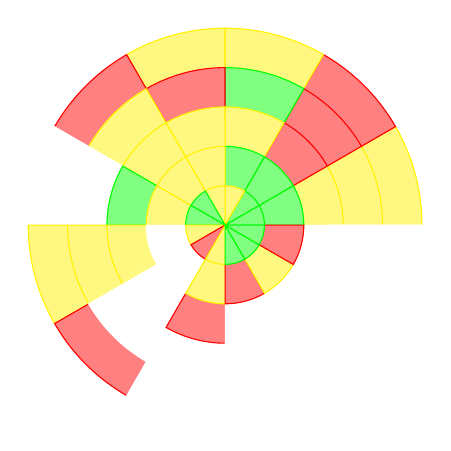
\begin{tikzpicture}[nodes = {font=\sffamily}]
      \foreach \color in {
            yellow,
            red,
            yellow,
            white,
            red,
            yellow,
            white,
            yellow,
            white,
            white,
            red,
            red,
        } {
        \ifx\color\empty\else
            \draw[fill={\color!50},draw={\color}] (0,0) -- (\angle:\radius)
              arc (\angle:\angle+30:\radius) -- cycle;
            \pgfmathparse{\angle+30}
            \xdef\angle{\pgfmathresult}
        \fi
        };
        \xdef\radius{2.5}
        \foreach \color in {
            yellow,
            red,
            yellow,
            yellow,
            red,
            white,
            yellow,
            red,
            white,
            white,
            white,
            white,
        } {
        \ifx\color\empty\else
            \draw[fill={\color!50},draw={\color}] (0,0) -- (\angle:\radius)
              arc (\angle:\angle+30:\radius) -- cycle;
            \pgfmathparse{\angle+30}
            \xdef\angle{\pgfmathresult}
        \fi
        };
        \xdef\radius{2}
        \foreach \color in {
            yellow,
            red,
            green,
            red,
            yellow,
            white,
            yellow,
            white,
            white,
            white,
            white,
            white,
        } {
        \ifx\color\empty\else
            \draw[fill={\color!50},draw={\color}] (0,0) -- (\angle:\radius)
              arc (\angle:\angle+30:\radius) -- cycle;
            \pgfmathparse{\angle+30}
            \xdef\angle{\pgfmathresult}
        \fi
        };
        \xdef\radius{1.5}
        \foreach \color in {
            yellow,
            red,
            yellow,
            yellow,
            yellow,
            green,
            yellow,
            white,
            red,
            white,
            white,
            white,
        } {
        \ifx\color\empty\else
            \draw[fill={\color!50},draw={\color}] (0,0) -- (\angle:\radius)
              arc (\angle:\angle+30:\radius) -- cycle;
            \pgfmathparse{\angle+30}
            \xdef\angle{\pgfmathresult}
        \fi
        };
        \xdef\radius{1}
        \foreach \color in {
            green,
            green,
            green,
            yellow,
            yellow,
            yellow,
            white,
            white,
            yellow,
            red,
            yellow,
            red,
        } {
        \ifx\color\empty\else
            \draw[fill={\color!50},draw={\color}] (0,0) -- (\angle:\radius)
              arc (\angle:\angle+30:\radius) -- cycle;
            \pgfmathparse{\angle+30}
            \xdef\angle{\pgfmathresult}
        \fi
        };
        \xdef\radius{0.5}
        \foreach \color in {
            green,
            green,
            yellow,
            yellow,
            green,
            green,
            yellow,
            red,
            yellow,
            green,
            green,
            green,
        } {
        \ifx\color\empty\else
            \draw[fill={\color!50},draw={\color}] (0,0) -- (\angle:\radius)
              arc (\angle:\angle+30:\radius) -- cycle;
            \pgfmathparse{\angle+30}
            \xdef\angle{\pgfmathresult}
        \fi
        };
    \end{tikzpicture}
\caption{Typical gateway coverage\cite{lorajambalaya}\label{fig:coverage}}
\begin{tabular}{r@{: }l r@{: }l}

\begin{tikzpicture}\draw[fill=green,line width=1pt]  circle(1ex);\end{tikzpicture} & Good\ Connection & 
\begin{tikzpicture}\draw[fill=yellow,line width=1pt]  circle(1ex);\end{tikzpicture} & Intermediate\ Connection\\

\begin{tikzpicture}\draw[fill=red,line width=1pt]  circle(1ex);\end{tikzpicture} & Bad\ Connection & 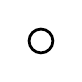
\begin{tikzpicture}\draw[fill=white,line width=1pt]  circle(1ex);\end{tikzpicture} & No\ Connection 
\end{tabular}
\end{figure}




Multi-hop networks, as represented in Fig~\ref{fig:meshtopology}, can be a solution to
the LoRaWAN scaling issues~\cite{8115756}.
Participants of the network do not directly send message to gateways, but
instead, pass messages to their neighboring nodes.
The use of a multi-hop routing protocol increases the reliability, the coverage
and allows to adapt to changes in the network (because of moving or failing nodes)
at the expense of higher energy consumption in the relaying motes.

Multi-hop routing protocols are de facto strong candidates for filling in the
routing tables for nodes deployed for large area monitoring
applications where gateways may be hard and costly to deploy and where blind
spots often arise.
This solution can potentially decrease the energy consumption of bordering
nodes that usually struggle to achieve successful communication in non-optimal
conditions.

\paragraph{}

Work to create a multi-hop routing protocol for LoRa multi-hop netowkrs has
already been done~\cite{8115756, DIAS2018424, 8856256, Abrardo_2019, duong2018},
but two main problems stand out from this similar work.

First, most studies consider that the motes are always-on and
neglect the problem of probable energy depletion.
LPWAN were designed to be used with battery operated motes that spend most of
his time sleeping and always-on motes go against that.
A solution to this first matter would be to use time-slotted channel access.
Synchronized nodes would be able to use a scheduling mechanism that tell them
when to wake-up to transmit or receive a packet.
This will put nodes in sleeping mode the rest of the time.
It also allows a deterministic access method to avoid collisions.

Second, these protocols only use a single channel.
This reduces network capacity and increases the risk of
interference.

\section{Approach}

Multi-hop routing solution already exists and can work on top of LoRa.
But until now LoRa multi-hop networks lacked a reliable and power efficient MAC protocol
to use in conjunction with routing protocols like the routing protocol for low power
and lossy networks (RPL).

The \emph{IEEE 802.15.4e} Time-Slotted Channel Hopping (TSCH) MAC protocol
has been designed for organizing reliable low power networks, we want to
investigate whether it would be a good candidate MAC protocol for LoRa based
multi-hop networks.
Using TSCH could actually solve many of the previous aforementioned issues.
First, TSCH uses channel hopping, making it resilient to external interference and
channel jamming and thus improving the reliability.
Second, TSCH uses synchronized motes and the notion of time slots to be able to organize
deterministic medium access, together with a schedule that will be designed to
minimize collisions and make the nodes sleep in slots in which no communication
need to take place.
An example of a schedule is Orchestra~\cite{duquennoy2015} that adapts to the
communication given by the routing protocol.
Adapting the TSCH protocol for LoRa would allow low power,
reliable and collision-free high-density networks, running over standards
multi-hop routing protocols.

\paragraph{}

This thesis aims to adapt the TSCH MAC protocol for LoRa.
thus bringing a reliable, long-range, and low power IPv6 multi-hop
solution to the LoRa ecosystem.

In order to achieve this, I will adapt the current TSCH implementation of
the Contiki operating system (OS) (originally developed for 802.15.4 compliant radio protocol)
to work with the longer delay induced by a low data-rate protocol like LoRa.
I will also implement a radio driver for the RN2483 in Contiki to have a
reliable LoRa radio driver working on the platform that I can adapt for my
needs.
In the end, I will have a fully working modified version of TSCH running on a
\emph{Zolertia RE-Mote} development board.

Testing my implementation in conjunction with RPL and the Orchestra schedule
for TSCH will successfully achieve multi-hop routing and thus demonstrating its
feasibility with LoRa.
An additional test ran over a jammed radio channel will show the reliability of
TSCH with LoRa.

\paragraph{}

Progress toward adapting TSCH for LoRa in~\cite{8847137} and~\cite{njomgang_2018},
has already been conducted in the previous year at \emph{VUB}.
This thesis builds on the combined efforts of previous work.

\section{Thesis Outline}

The next chapter will give the background information and context needed to
understand the building blocks to achieve my end goal.
It will also give an overview of the related work on the subject of
LoRa multi-hop communications.
Chapter \ref{section:radio} gives the implementation details of realising a driver for the
RN2483 in Contiki OS and the experimentation with the driver.
Chapter \ref{section:tsch} gives instructions and guidelines for adapting and
operating TSCH with LoRa on Contiki OS and reports on the different testing I conducted.
Chapter \ref{section:conclusion} will conclude the work by summarizing it and
will suggest possible futur research on the subject.
